\section{Structure}\label{sec:Structure}
For the simulation environment to be useful some basic functionality is needed. The simulation should be easy to setup and adjust if needed. 
Furthermore an easy way to view the result of the simulation is needed such that necessary adjustments can easily be made based on the result.
Based on this the design phase can be split in to three parts:

\begin{enumerate}
	\item Initialization
	\item Simulation
	\item Result
\end{enumerate}

To solve the non-linear equations obtained for the free flow channel model in subsection \ref{subse:open_channel} the Preissman scheme is utilized. This scheme explained in detail in  

The following will go into details of the design off, and the considerations made during the design phase, of the three above points.
As mentioned in section \ref{ch:simulation_solution_and_limitation} a solution to minimize flow and concentrate variations could be insertion of one or more tanks in the sewer network. 

The first overall thing to consider is the composition of components desired to simulate. Making the simulation able to simulate different setups than the one shown in figure \ref{fig:kloakgrid_simplified}. For this a universal setup procedure, where different sizes of pipes with different slopes with selective side input, is needed. 
The second thing to consider is that the environment should be brought to a steady state before the simulation starts. The reason for this is that if a linearized approach to the MPC scheme is chosen a linear model is necessary.  

\subsection*{Initialization} 
The initialization process can be split in to further parts where the setup of the desired pipe system is performed such that the the system is simulated with the components in the right order.
Secondly the system should be brought in to a steady state from which the simulation can start. A simple system setup, consisting of a MATLAB function where the order of the component decides the place in the system to be simulated, is decided upon. An example of the setup procedure is shown in figure \ref{fig:sys_setup}  

\begin{figure}[H]
\centering
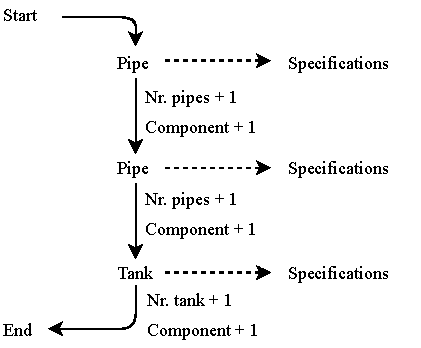
\includegraphics[width=0.55 \textwidth]{report/simulation/pictures/sys_setup.pdf}
\caption{Setup scheme of system order initiation}
\label{fig:sys_setup}
\end{figure}

The necessary specifications entered for pipe and tank respectively should as a minimum be the      